\documentclass{article}
\usepackage{graphicx} % Required for inserting images
\usepackage{authblk}

\title{HLoRA: Hierarchical Low-Rank Adaption for Multi-task Large Language Models}
\author[1]{Simen Eide}
\author[2]{Arnoldo Frigessi}
\affil[1]{University of Oslo, Schibsted}
\affil[1]{University of Oslo}
\date{March 2024}

\usepackage[
backend=biber,
style=alphabetic,
sorting=ynt
]{biblatex}
\usepackage{amsmath}
\usepackage{amssymb}
\newcommand{\R}{\mathbb{R}}
\usepackage{booktabs}
\addbibresource{My Library.bib}

\begin{document}

\maketitle
\abstract{Lorem Ipsum}

\section{Introduction}
Large Language Models (LLM) have become a popular model architechture for solving a wide range of text problems. LLMs are typically pretrained on a large and diverse dataset, and then fine-tuned on a specific task. The fine-tuning process is often done by maximizing the next token log likelihood of the task-specific dataset, and the resulting model is then used to make predictions and generations on new data. A popular fine-tuning method is Low-Rank Adaption (LoRA), which reduces the number of trainable parameters by up to 10'000 times and the GPU memory requirement by 3 times, while still outperforming other fine-tuning techniques (\cite{hu_lora_2021}).

When applying fine-tuning of LLMs to problems, the practitioner often wants to solve multiple similar tasks at the same time. 
For instance, a news organization might want to use an LLM to generate various textual elements for a given article such as headlines, keywords, and summaries, all based on the main body of the text. This would involve fine-tuning the model for each of these distinct but related tasks.
Similarly, a customer service chatbot might need to be fine-tuned to handle inquiries across a range of topics, such as product information, order status, and troubleshooting. Additionally, the chatbot might need to adapt its responses based on the user's tone or the formality of the conversation, requiring further fine-tuning.
In a more creative context, a scriptwriting AI might be fine-tuned to generate dialogues for different characters in a movie, each with their unique style and vocabulary. This would involve fine-tuning the model for each character, a set of related but distinct tasks.

In these cases, the practitioner can either (1) train one model for each task separately, or (2) train one model for all tasks and condition the specific output wanted (e.g \cite{Raffel2019}).
There is a trade-off between these two approaches: Train each task separately and the model will be able to specialize on each task, but it may suffer from limited data for each task. Train one model for all tasks, and the model will be able to share information between tasks, but it may not be able to specialize on each task due to limited model capacity.

This paper suggests a way to circumvent these trade-offs and presents a generalization of the two LoRA fine-tuning methods for multi-task problems, which we call Hierarchical Low-Rank Adaption method (HLoRA).
The Hierarchical LoRA method allows tasks to share information between each other through sharing a set of global hierarchical prior parameters. 
This means that tasks with little data can benefit from the global structure of the related tasks, while tasks with more data can specialize on their specific task.
We show in Section \ref{sec:hlora} that HLoRA can be seen as a generalization of the two approaches above.

To test our method, we evaluate the Hierarchical LoRA method on the next token generation problem of parliament speeches letting each parliament representative be a task. In our setting, HLoRA is superior to both conventional approaches above and suggest a way to mitigate the trade-off between the two.
% Write something about how easy it is to implement and how it can be used in practice?

The paper is organized as follows: Section \ref{sec:related_works} presents related works, Section \ref{sec:method} presents the Hierarchical LoRA method, (...)

% Should this fact be added somewhere?
% If the D tasks are more similar to eachother than the pretraining corpus, the optimal parameters $\hat{\theta}_d$ should share some information during training in order to maximize their likelihood.


\section{Related works} \label{sec:related_works}
%%%%%%%%%%%%%%%%%%%%%%%%%%%%%%%%%%

\subsection{Multi-task Learning}
Multi-task Learning \cite{caruana_multitask_nodate} is a popular machine learning approach for training one model on multiple tasks. A common approach is to share the lower layers of a neural network between tasks, and have separate output layers for each task. Our paper focuses on a different approach, where we share information between tasks through a hierarchical prior over the task-specific parameters.

\subsection{Finetuning methods}
A popular approach to finetuning neural networks involves adjusting only the top layer (or the n top layers) of a pre-trained neural network (e.g. \cite{yosinski2014transferable}). These techniques observe that features learned in the lower layers of the network are general and transferable, while the top layers are more task-specific. This approach has been widely adopted in neural networks. However, we focus on the LoRA method, which allows us to train a low rank decomposition of the entire network.

There are several variations of the LoRA algorithm. The Sparse Mixture of Low Rank Adapters (SIRA) \cite{zhu_sira_2023}, for instance, creates a Mixture of Expert on the low-rank parameters. Another variation, the Weight Decomposed Low-Rank Adaption (DoRA) \cite{hayou_lora_2024}, decomposes the low-rank parameters into scale and unit norm direction parameters. There's also the Efficient Low Rank Adaption (LoRA+) \cite{hayou_lora_2024}, which improves the existing LoRA optimization algorithm by adjusting the learning rate of the low-rank parameters.
All these methods are designed to improve the performance of the LoRA algorithm, and can be used in conjunction with the Hierarchical LoRA method.

%%%%%%%%%%%%%%%%%%%%%%%%%%%%%%%%%%
\section{Method: Hierarchical LLM} \label{sec:method}
%%%%%%%%%%%%%%%%%%%%%%%%%%%%%%%%%%
This section describes the Hierarchical LoRA method for multi-task problems. We start by defining the task and data structure, and then introduce the pretrained autoregressive language model. We then describe the LoRA method, and finally present our Hierarchical LoRA model.

\subsection{Task and Data Structure}
We define our study across $D$ distinct tasks, denoted as $d=1,2,...,D$. For each task $d$, we have a dataset $\mathcal{D}_d$ containing $N_d$ documents, with each document consisting of a sequence of $W_n$ tokens. This dataset structure can be formally represented as:

\begin{equation} \label{eq:data}
\mathcal{D} = \{ \mathcal{D}_d \}_{d=1}^D  =  \{ \{ w_{d,n,1:W_n} \}_{n=1}^{N_d} \}_{d=1}^D
\end{equation}
%
In this notation, $w_{d,n,1:W_n}$ represents the token sequence in the $n^{th}$ document of the $d^{th}$ task. For simplification in subsequent discussions, we will omit the indices $d$ and $n$ when their reference is evident from the context.

\subsection{Pretrained Autoregressive Language Model}
Our foundational model is a pretrained autoregressive language model, denoted by its parameters $\theta_{full}$ and its architecture, referred to as a Large Language Model ($LLM$). The parameters $\theta_{full}$ has been obtained from pretraining on a large and diverse dataset, distinct from our current dataset $\mathcal{D}$. The model's probability distribution is given by:
The model's probability distribution is given by:

\begin{equation} \label{eq:LLMprob}
P(w_{1:W} | \theta_{full}) = \prod_{i=1}^{W-1} LLM(w_{i+1} | w_{1:i})
\end{equation}
%
where $LLM(w_{i+1} | w_{1:i})$ is the probability of the next token $w_{i+1}$ given the previous tokens $w_{1:i}$ in the document.
We omit to write $\theta_{full}$ explicitly in the model, as the autoregressive language model always depend on these parameters.

\subsection{Low-Rank Adaption (LoRA)}
A Large Language Model contains many linear layers, and the LoRA method reduces the number of trainable parameters by reparameterizing the weight parameters ($W \in \R^{n_1 \times n_2}$) of these layers into the original pretrained weights $W_{full}$ and a low-rank decomposition $A$ and $B$ (\cite{hayou_lora_2024}):
\begin{equation} \label{eq:LoRA}
    W = W_{full} + \frac{\alpha}{r} BA 
\end{equation}
%
where $W_{full} \in \R^{n_1 \times n_2}$ is the original pretrained weight, $B \in \R^{n_1 \times r}$ and $A \in \R^{r \times n_2}$ are the low-rank factors, $r \ll \text{min}(n_1, n_2)$ is the low rank dimension and $\alpha$ is a scaling hyperparameter.

During LoRA fine-tuning, the low-rank factors $A$ and $B$ are learned from data as normal parameter matricies, while the original pretrained weights $W_{full}$ are kept fixed.

\subsection{The Hierarchical LoRA model} \label{sec:hlora}
In the hierarchical LoRA model, we introduce a LoRA parameter set for each task $d$, denoted as $\theta_d$, containing all the low-rank decomposition matricies $A$ and $B$ from each decomposed layer in the Large Language Model. The likelihood of the data $\mathcal{D}$ given the task parameters $\theta_{1:D}$ is then given by (combining equation \ref{eq:data} and \ref{eq:LLMprob}):
\begin{equation} \label{eq:lik}
    \text{L}(\mathcal{D} | \theta_1, \theta_2, \ldots, \theta_D) = \prod_{d=1}^D L(\mathcal{D}_d | \theta_d) = \prod_{d=1}^D \prod_{n=1}^{N_d} \prod_{i=1}^{W_n-1} \text{LLM}(w_{d,n,i+1} | w_{d,n,1:i}; \theta_d)
\end{equation}
%
%
Each task will share some information with each other, and we model this by introducing a Gaussian hierarchical prior over the task parameters $\theta_{1:D}$, given by
\begin{equation} \label{eq:prior}
    P(\theta_{1:D} | \Theta, \tau ) = \prod_{d=1}^D N(\theta_d ; \Theta, \frac{1}{\tau} I)
\end{equation}
%
where $\Theta$ is a set of hierarchical mean parameters, $I$ is a unit diagonal matrix and $\tau \geq 0$ is a scalar precision hyperparameter controlling how similar task parameters $\theta_d$ should be to the hierarchical mean parameters $\Theta$.
We let $\Theta$ have a uniform prior (i.e. $P(\Theta) = 1$).

The posterior distribution of the hierarchical model is then given by combining equation \ref{eq:lik} and \ref{eq:prior}:
\begin{equation} \label{eq:posterior}
    P(\theta_{1:D} | \mathcal{D}, \tau) \propto \prod_{d=1}^D \text{L}(\mathcal{D}_d | \theta_d) \cdot P(\theta_d | \Theta, \tau)
\end{equation}
%
%
The precision hyperparameter $\tau$ controls how much the task parameters $\theta_d$ should be allowed to deviate from the hierarchical mean parameters $\Theta$. 
This is essentially a proxy for how much structure and information the tasks share with each other, and should be set by the practitioner based on her's prior knowledge.

The resulting HLoRA model balances each task based on its data size and similarity to the other tasks: If a task has few data points, the posterior in equation \ref{eq:posterior} will be dominated by the prior term and the task parameters will be close to the global hierarchical parameters and borrow information and structure from these. On the other hand, if a task has a lot of data points, the likelihood will dominate the posterior and the task parameters will be allowed to learn more about the specific task and rely less on the hierarchical parameters.

The hierarchical LoRA model can be seen as a generalization of the two conventional approaches for multi-task problems:
If we let $\tau$ go to zero, the probability distributyion of the prior (eq. \ref{eq:prior}) will become a flat uniform prior and the problem will be equivalent to training each task independently. On the other hand, if we let $\tau$ go to infinity, the prior will become a strong constraint on the task parameters not allowing them to deviate from the global parameters, and the problem will be equivalent to training one model for all tasks.

\subsection{Optimization}
Given a precision hyperparameter, we want to find the maximum a posteriori (MAP) estimate of the hierarchical model. 
We will do this by using AdamW (\cite{adamW}), a gradient-based optimization algorithm, optimizing over the task parameters $\theta_{1:D}$ and the hierarchical mean parameters $\Theta$ simultaneously optimizing the likelihood and the prior in equation \ref{eq:posterior}.
This implies that the task parameters with have gradients both towards minimizing the convential LLM loss and the hierarchical mean parameters. The hierarchical mean parameters $\Theta$ will have gradients towards the average of the task parameters, and learn to represent the global structure of the tasks after the task parameters have been partly optimized.

An important observation is that the gradient of the prior term in equation \ref{eq:posterior} is proportional to the precision hyperparameter $\tau$. This means that the optimization will more steps to converge for larger values of $\tau$, as the task parameters will be more constrained towards the hierarchical mean parameters.
Therefore, we adjust the learning rate of the AdamW optimizer to be proportional to the precision hyperparameter $\tau$, and we find in informal tests that this cause the optimizations to converge at a similar rate for different values of $\tau$.

\section{Experimental setup}
%%%%%%%%%%%%%%%%%%%%%%%%%%%%%%%%%%
% Use the Talk of Norway Dataset consisting of speeches of Norwegian parliament politicians. We will consider different speakers of this dataset as different tasks, and see how the hierarchical model can benefit from sharing information between these tasks.
% add figure of the dataset distribution in file training_lengths.png
\begin{figure}[h] \label{fig:task_len}
    \centering
    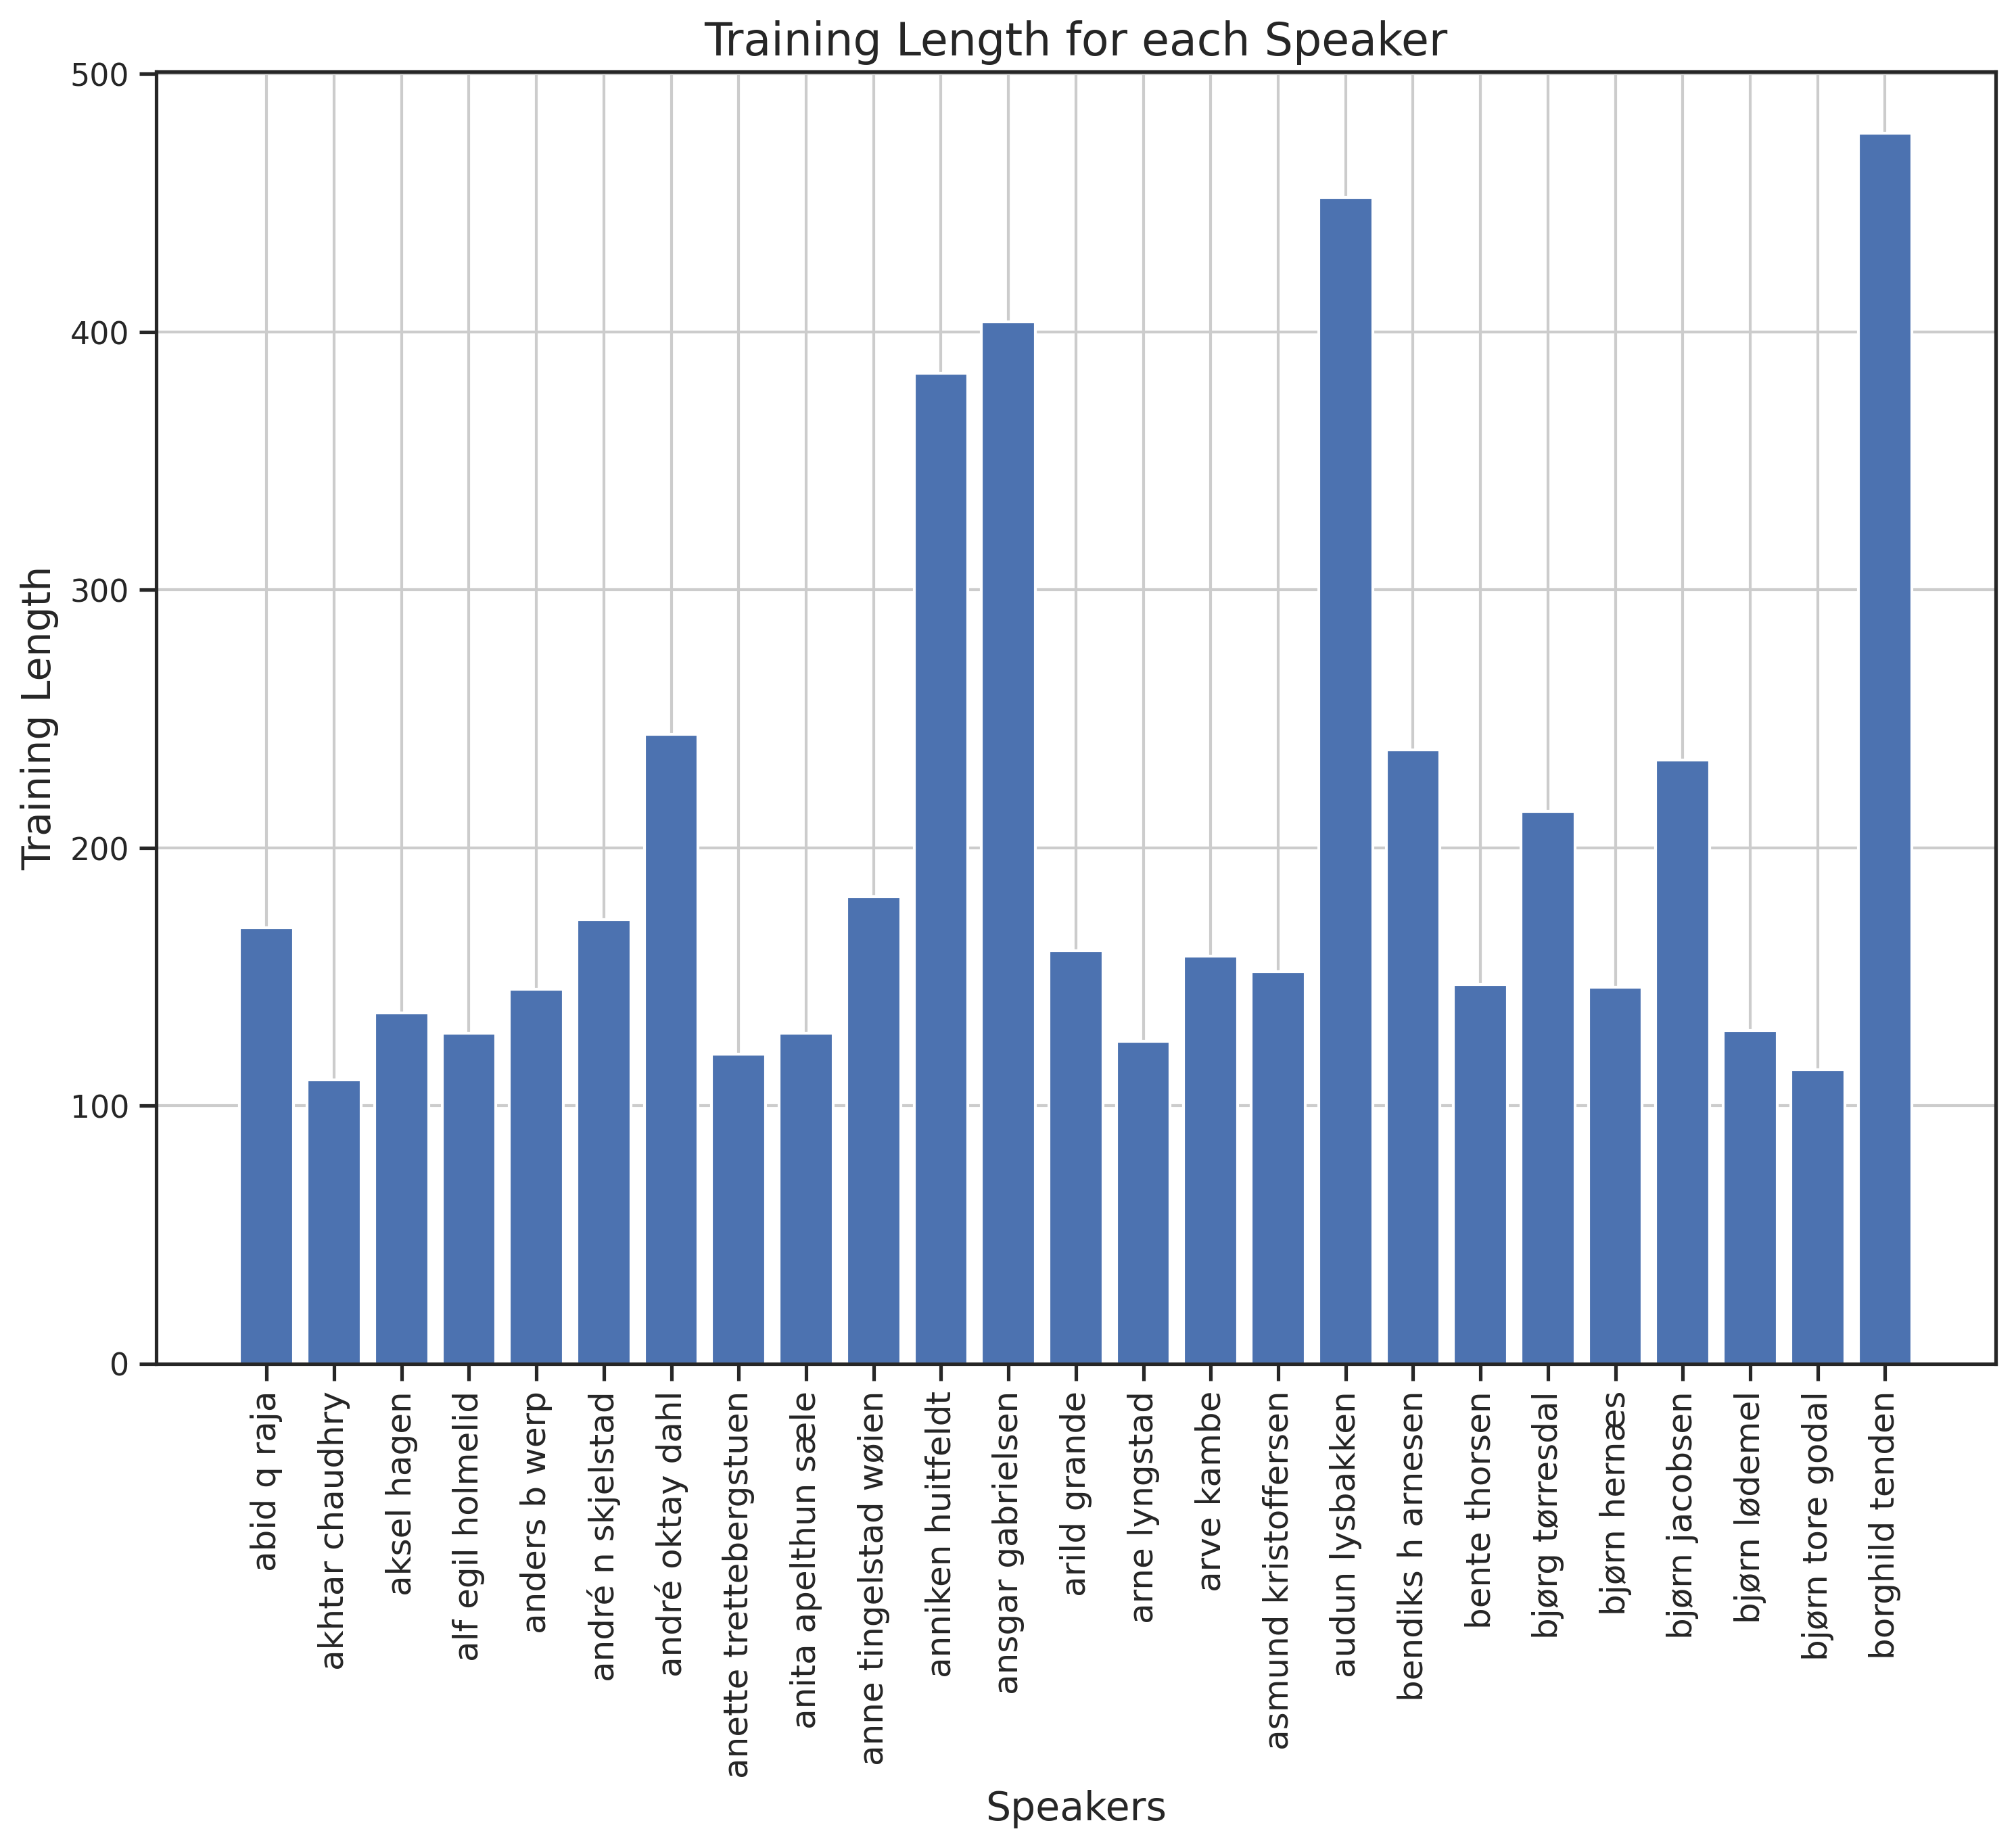
\includegraphics[width=\textwidth]{figures/training_lengths.png}
    \caption{Number of training examples for each task}
    \label{fig:training_lengths}
\end{figure}
% As base model, use opt-350m as it is predominantly trained on English, and only has seen a small amount of Norwegian data from the commoncrawls dataset.
To test our method, we optimize the model with a range of different precision hyperparameters $\tau$, and evaluate the model's perplexity on the test set for each task.
We use the Talk of Norway Dataset \cite{lapponi_talk_2018}, which consists of speeches of Norwegian parliament politicians. Each speaker will come from different political parties and geographical areas, but the tasks will still share a common domain. Therefore, we can consider different speakers of this dataset as different tasks. Specifically, we select chronologically the 25 first speakers that have above 100 speeches in the dataset.
This gives us a total of 25 tasks with samples ranging from 110 to 477 documents, and an average of 202 documents per task.
The distibution of samples per task can be seen in Figure \ref{fig:task_len}.
We leave 33\% of the data for the test set.

We select a model that has been pretrained on a large and diverse dataset, but has not seen the specific tasks that we want to evaluate it on. We will use the `opt-350m` model \cite{zhang_opt_2022}, which is predominantly trained on English, and has only seen a small amount of Norwegian data from the CommonCrawls dataset.

\section{Results}
%%%%%%%%%%%%%%%%%%%%%%%%%%%%%%%%%%
The overall results of the hierarchical LoRA model on the Talk of Norway Dataset are shown in Table \ref{tbl:results} and Figure \ref{fig:results_plot}. We see that the model achieves the best test perplexity of 12.82 when using a precision parameter of $100$. The improvement is largest from training the models independently ($\tau = 0$), and smaller when comparing to the limiting case when all task specific model parameters are constraint to be equal ($\tau=10000$).

\begin{table}[h] \label{tbl:results}
    \centering
    \begin{tabular}{ccc}
        \toprule
        Learning Rate & Precision ($\tau$) & Test Perplexity \\
        \midrule
            $10^{-4}$ &              0 &                 16.80 \\
            $10^{-5}$ &       $10^{0}$ &                 16.59 \\
            $10^{-4}$ &       $10^{1}$ &                 12.85 \\
            $10^{-3}$ &       $10^{2}$ &                 \textbf{12.82} \\
            $10^{-2}$ &       $10^{3}$ &                 13.26 \\
            $10^{-1}$ &       $10^{4}$ &                 13.91 \\
        \bottomrule
        \end{tabular}
        \caption{Empirical results of the hierarchical LORA finetuned on the three tasks. The perplexity is calculated on the test set.}
    \end{table}

\begin{figure}[ht]
    \centering
    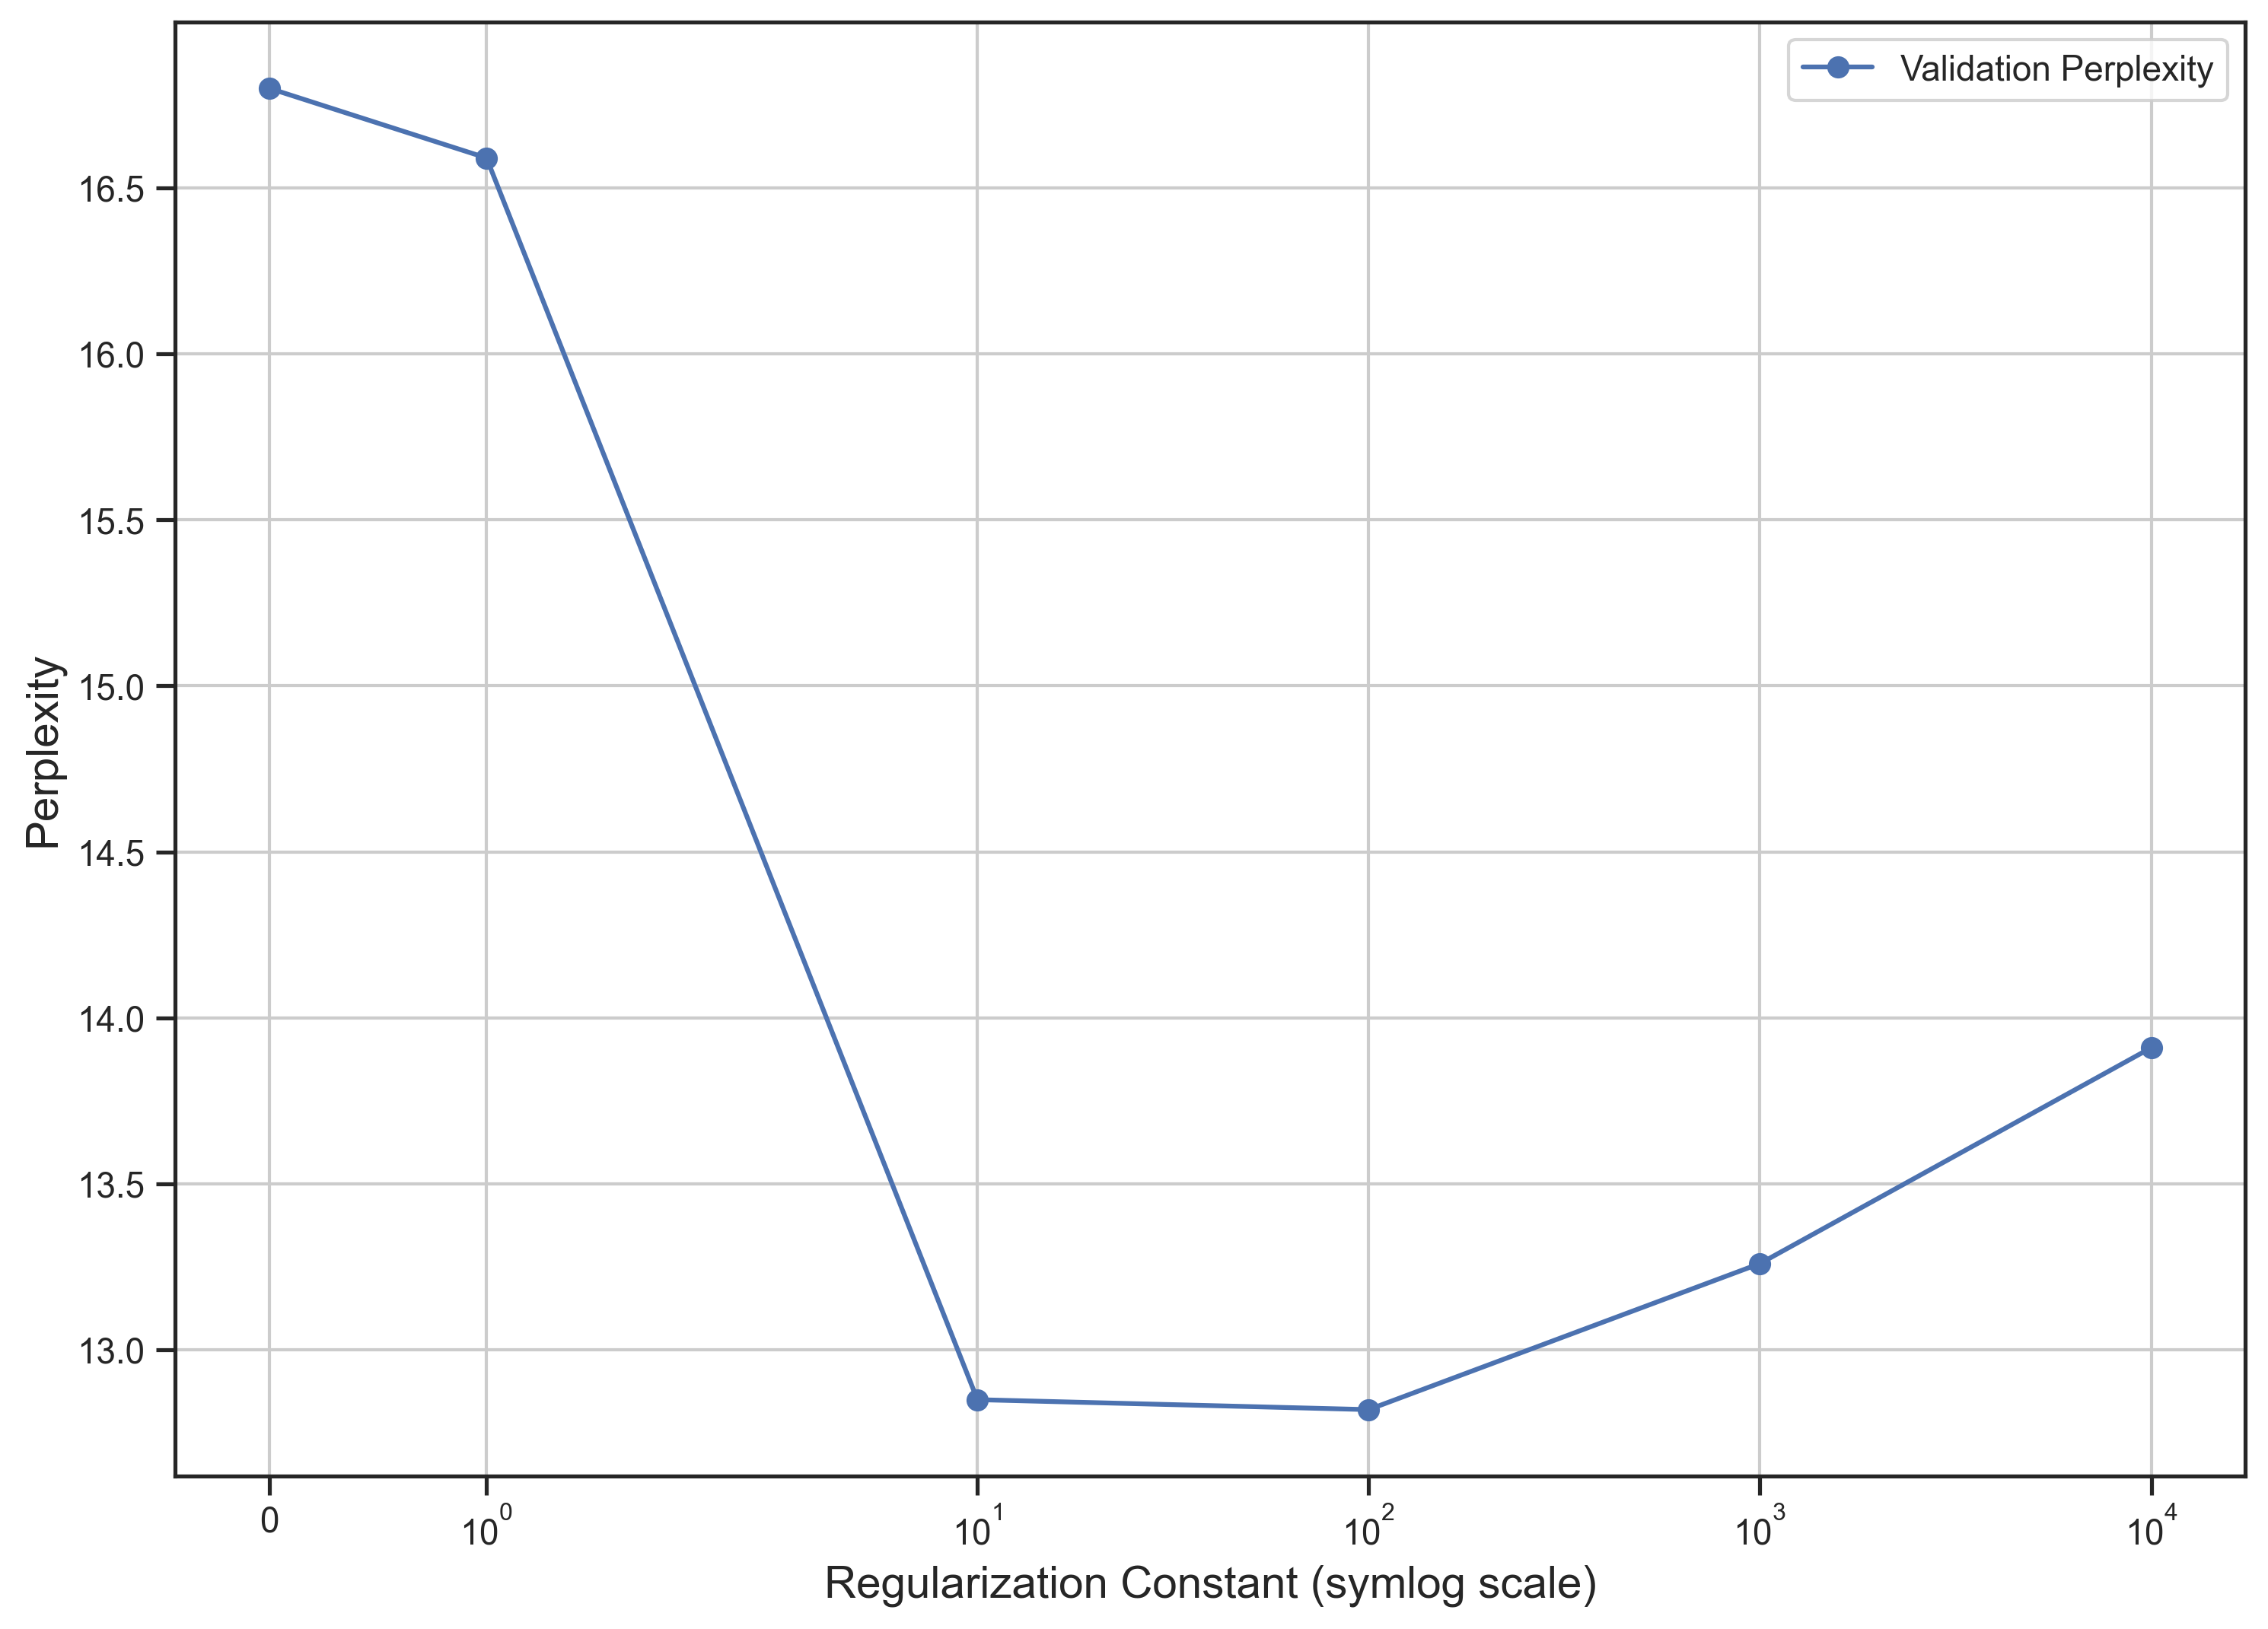
\includegraphics[width=\textwidth]{figures/results_plot.png}
    \caption{Plot of Precision vs Perplexity. The thick black line is the overall test perplexity over all tasks, and the thinner grey lines are the test perplexity for each individual task.}
    \label{fig:results_plot}
\end{figure}

If we consider each task separately (Table \ref{tbl:task_perplexities}), we see that all tasks benefit from a hierarchical model compared to both the case when all models are trained independently ($\tau = 0$) and the limiting case when all task specific model parameters are constraint to be equal ($\tau=10000$).
Figure \ref{fig:relative_improvement} shows the relative improvement of each task when using the hierarchical model compared to the two cases versus their training data size. There is an indication that the improvement from training separately is larger for tasks with less data, and we do not see this for the "one model" case.
A precision parameter of $100$ gives the best perplexity for all our tasks.

\begin{figure}[h]
    \centering
    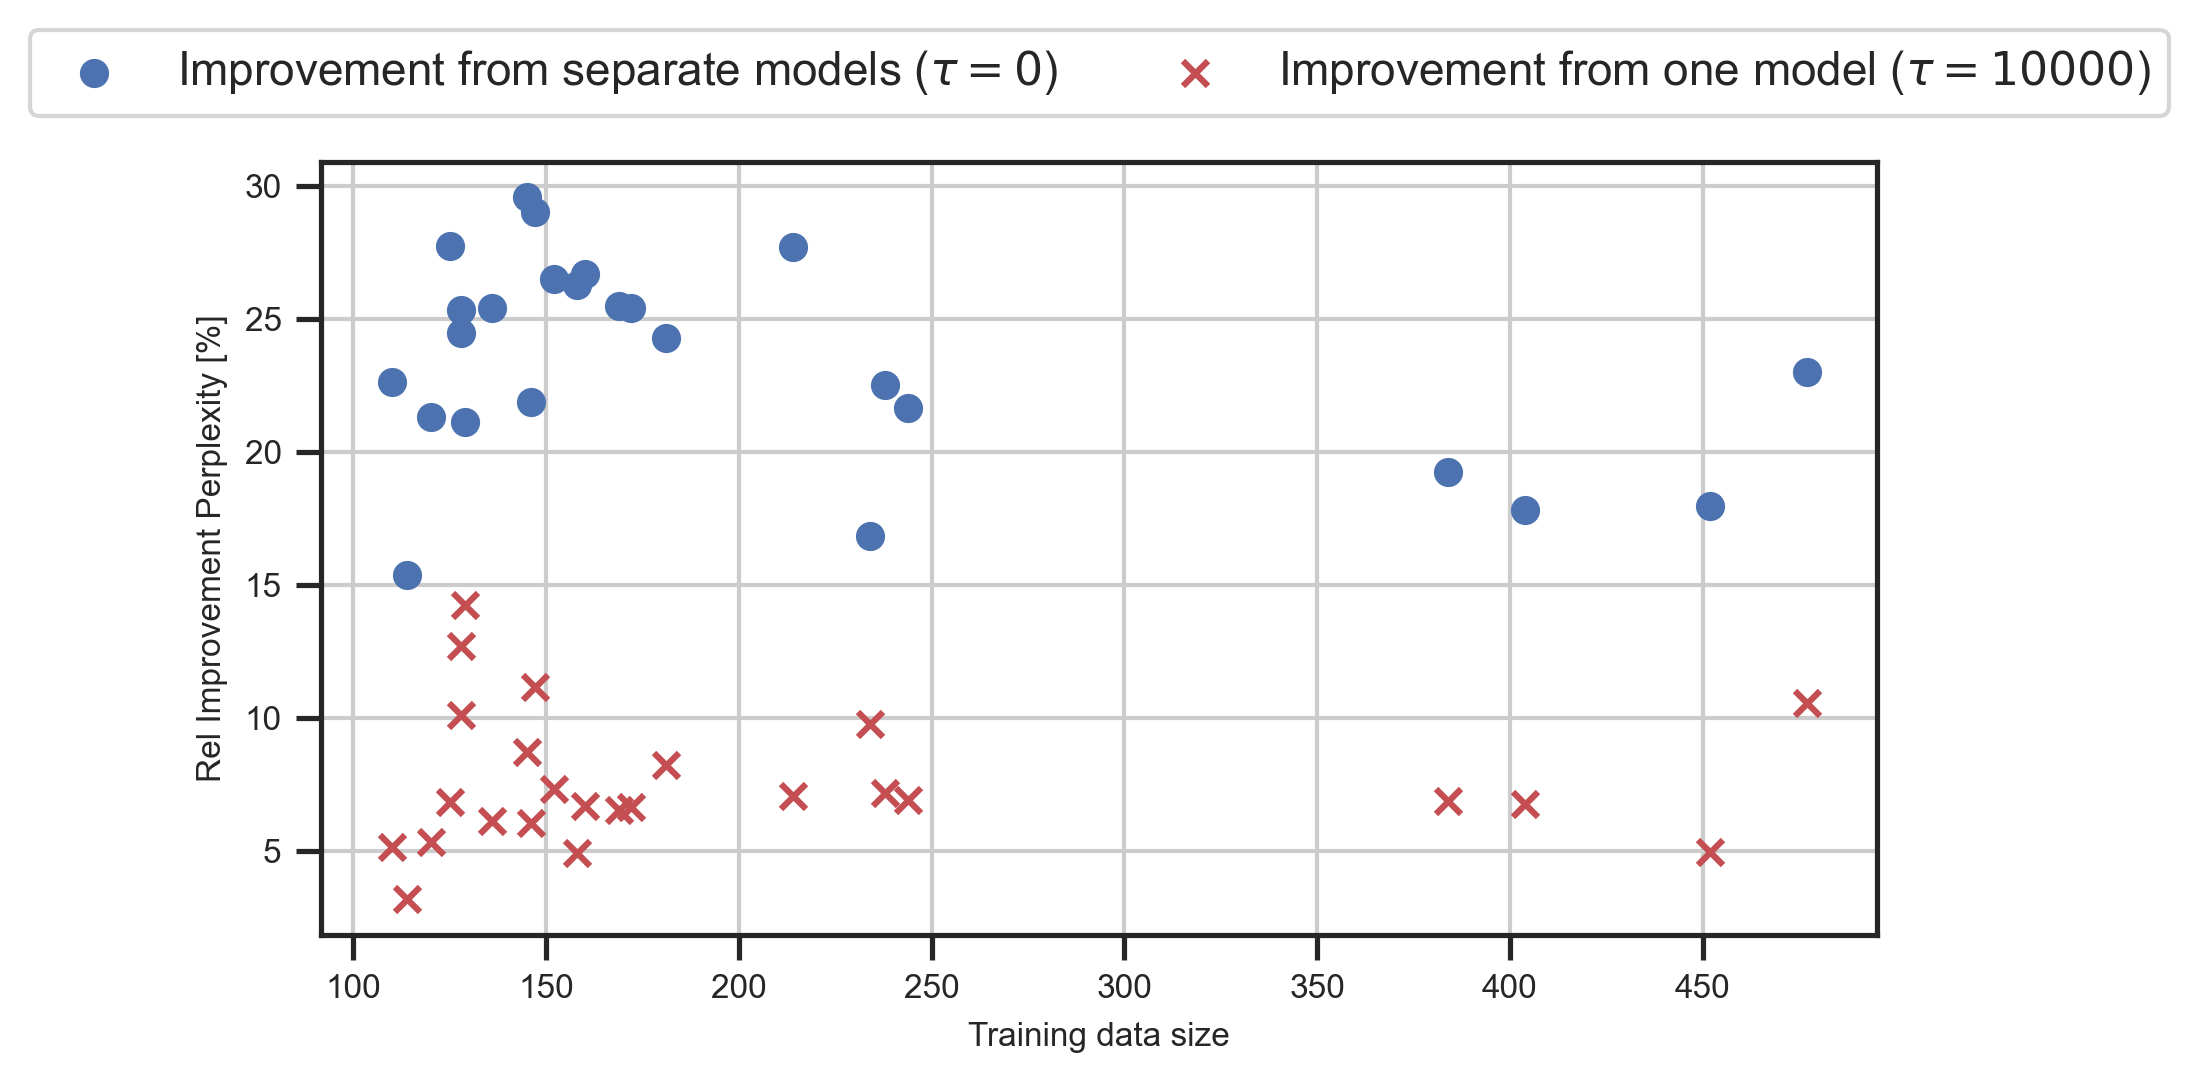
\includegraphics[width=\textwidth]{figures/relative_improvement_combined.png}
    \caption{Task dataset size versus the relative improvement in perplexity of the best performing hierarchical model ($\tau = 100$) compared to the case when all models are trained independently ($\tau = 0$) in blue, and compared to the limiting case when all task specific model parameters are constraint to be equal ($\tau=10000$) in red. 
    The figure shows that all tasks benefit from sharing parameters with the global model, and indicates that the tasks with less data benefit more than the tasks with more data.}
    \label{fig:relative_improvement}
\end{figure}

\section{Discussion}
%%%%%%%%%%%%%%%%%%%%%%%%%%%%%%%%%%
Our results in Figure \ref{fig:results_plot} show that the hierarchical LoRA model can improve the test perplexity for all tasks compared to both training the models independently and training one model for all tasks. This confirms our hypothesis that HLoRA can be a useful method for multi-task problems, and that it can mitigate the trade-off between training each task separately and training one model for all tasks.

We observe in Figure \ref{fig:weights_vs_datalen} that the distance between the task parameters and the global prior increases with increasing task dataset size. This is as expected in a hierarchical model, as tasks with more data will have a larger likelihood term in the posterior and will be allowed to specialize more on their specific task during training.

We find no relationship between dataset size and the final perplexity (Figure \ref{fig:absolute_improvement}). One could expect that tasks with more data are able to learn more about their specific task and achieve a lower perplexity, but this is not the case in our experiments. There are many other factors that can influence the final perplexity, and we believe that this is the reason in our case.
However, when considering the relative improvement of the best performing model, the results in Figure \ref{fig:relative_improvement} show tasks with less data may benefit more than the tasks with more data. Although a weak signal, this is an expected result, as the hierarchical model allows tasks with little data to borrow information and structure from the global model, while tasks with more data can specialize on their specific task.

\begin{figure}
    \centering
    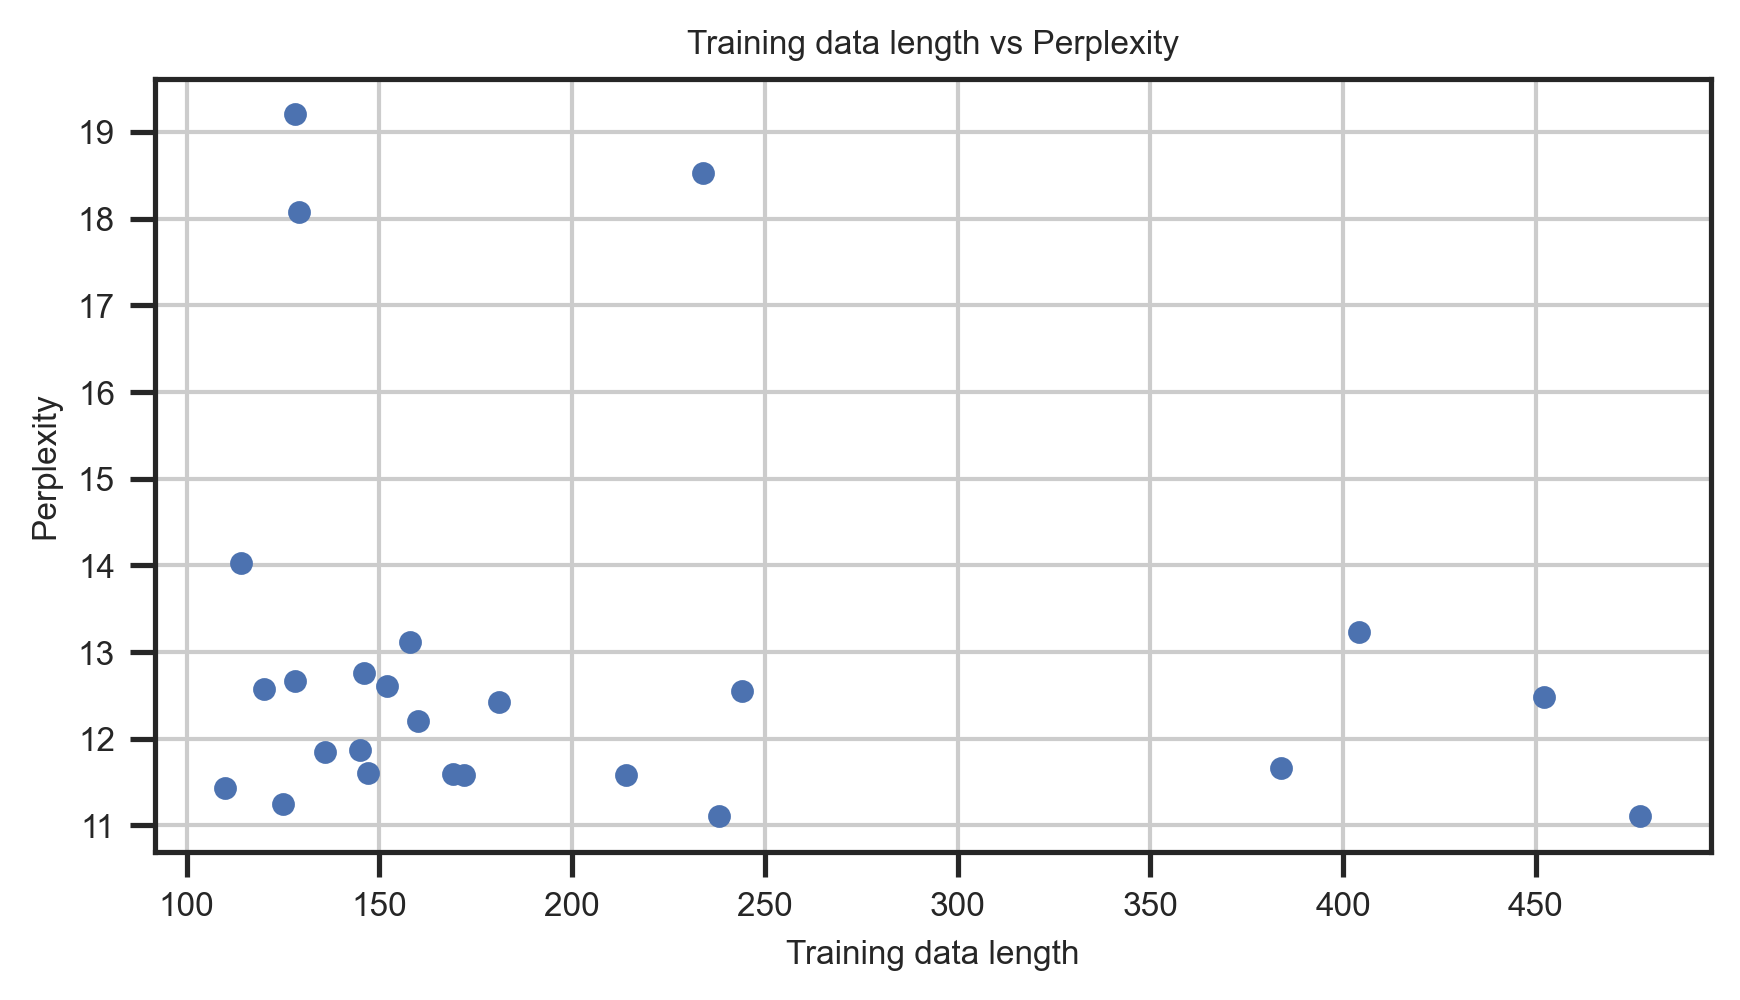
\includegraphics[width=\textwidth]{figures/trainingsize_vs_perplexity.png}
    \caption{Training size vs perplexity of the best performing hierarchical model ($\tau = 100$). The figure shows that there is no strong relationship between dataset size and final perplexity.}
    \label{fig:absolute_improvement}
\end{figure}

% Discuss overall result
% Fetch perplexity for each task and discuss how it improves results significantly for some tasks (less data?), and less larger data tasks.
% Give some advice on how to use this method in practice.

\begin{figure}[h]
    \centering
    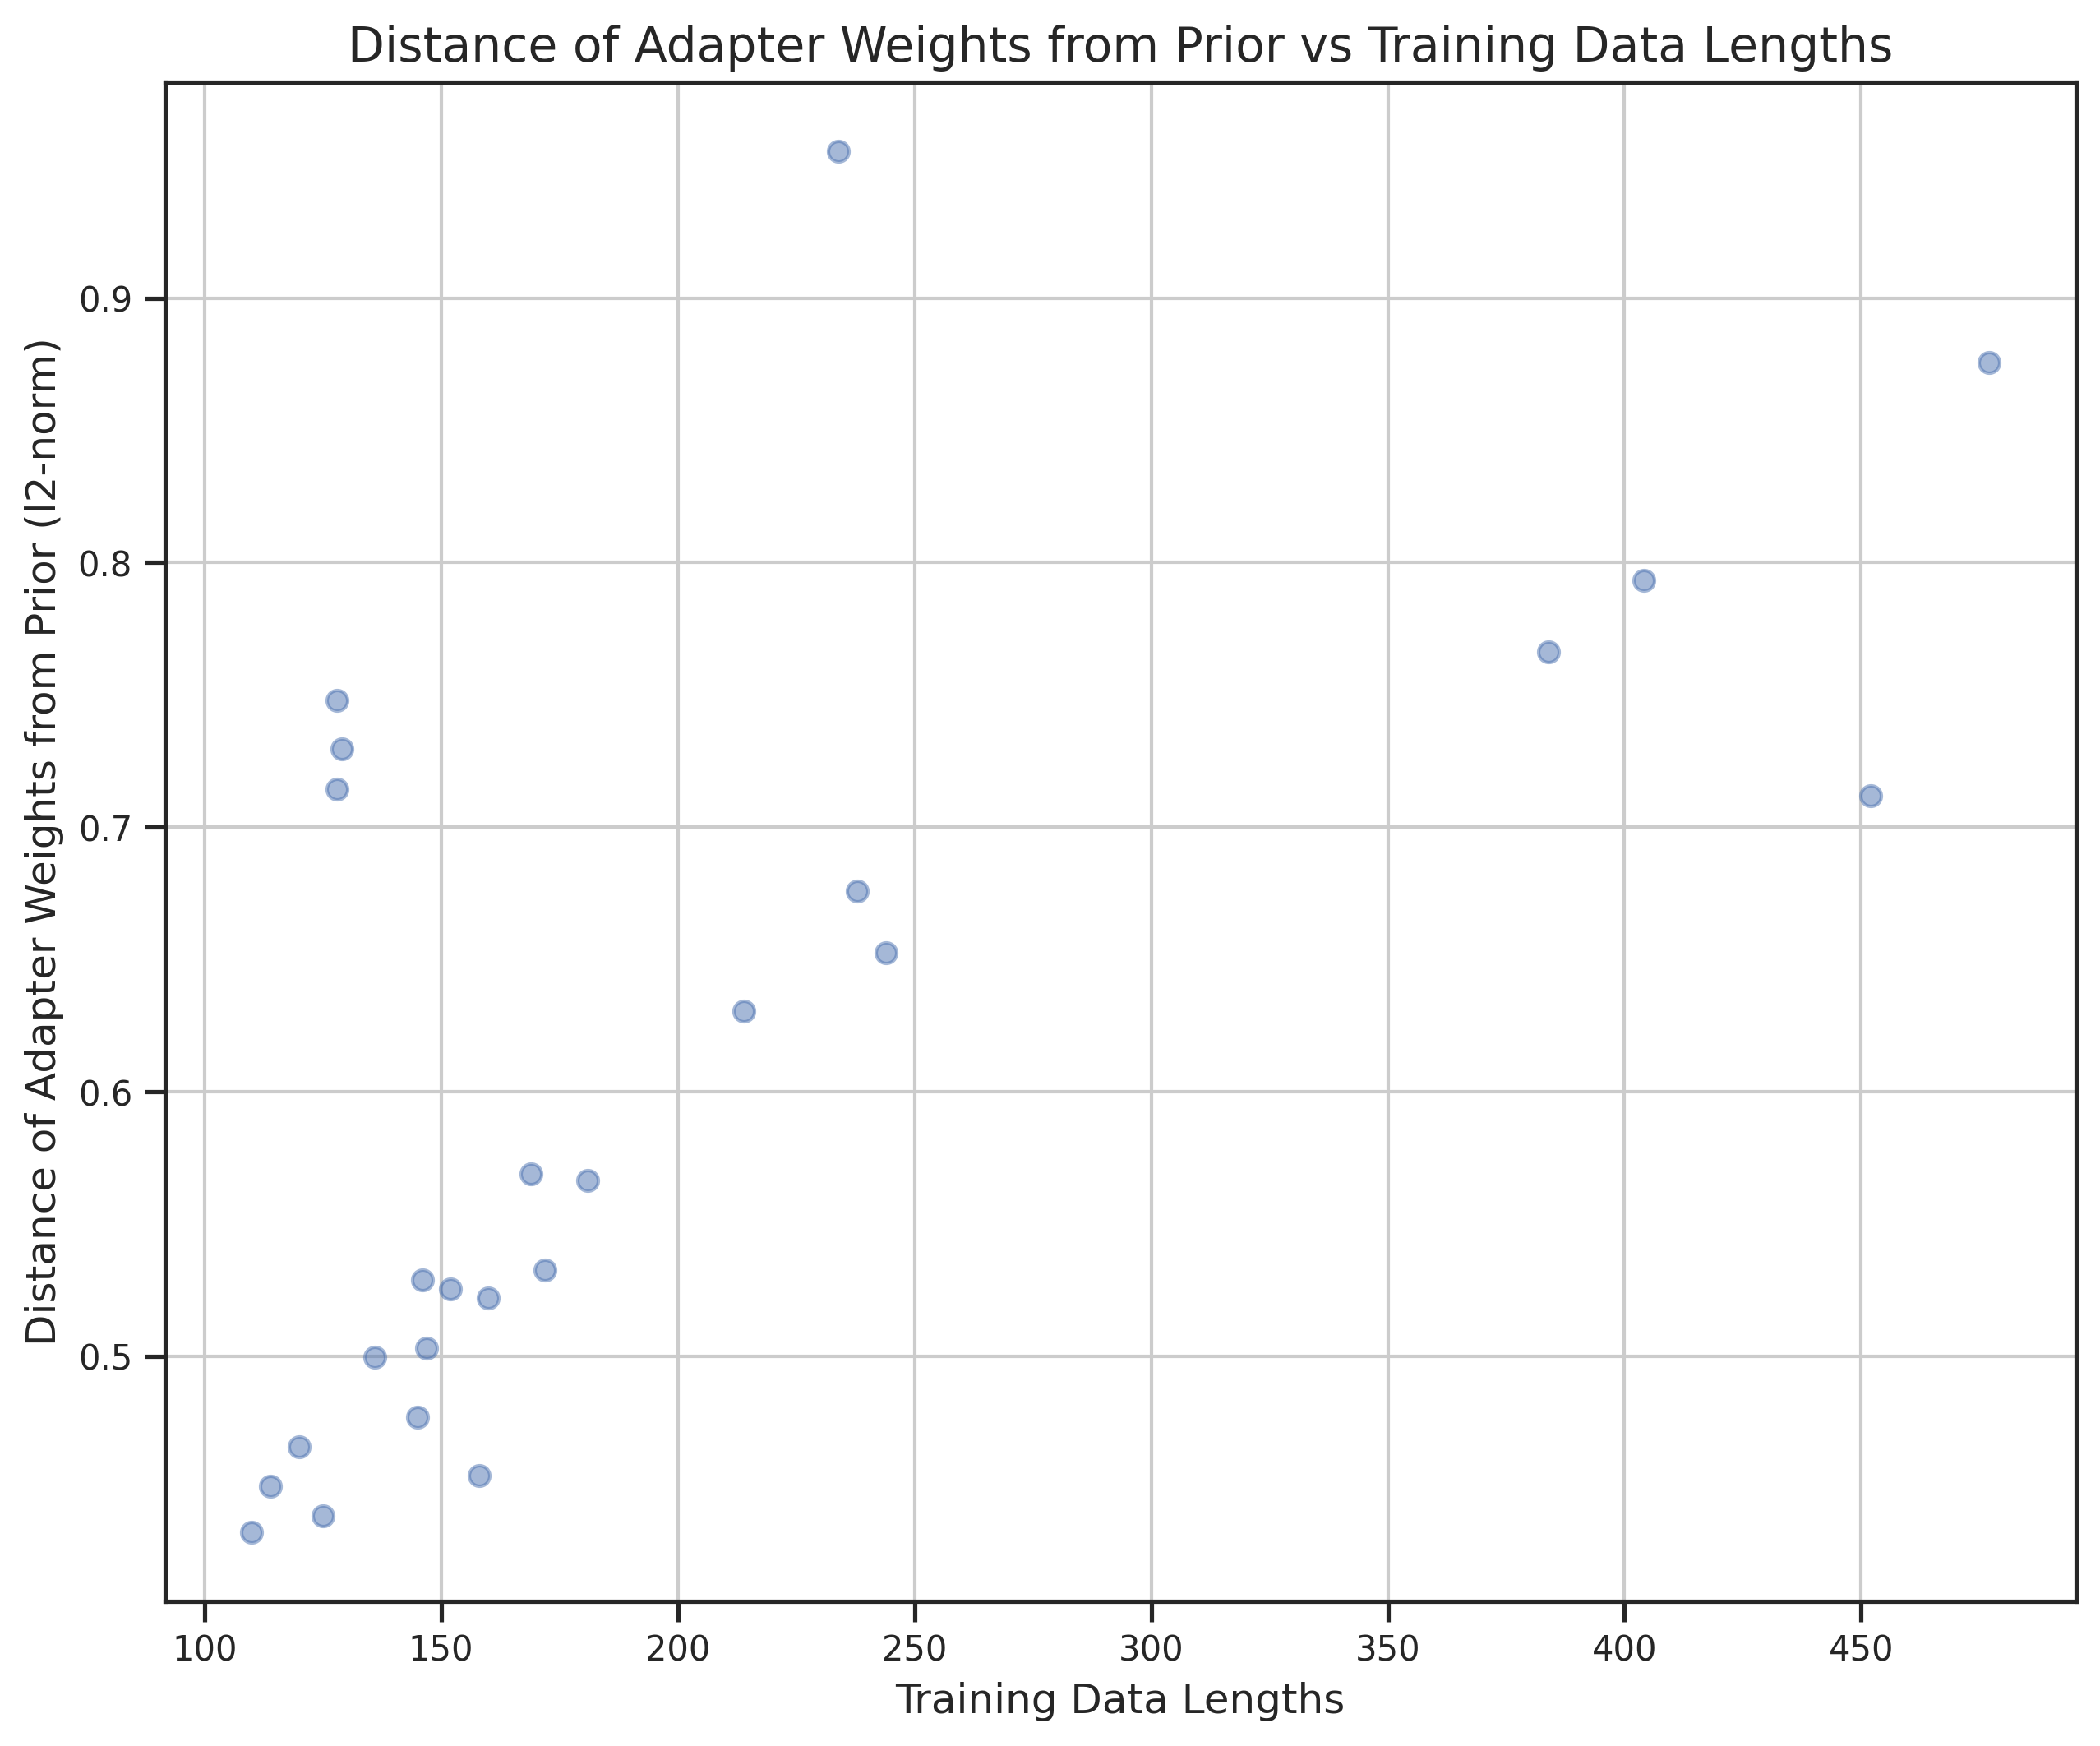
\includegraphics[width=\textwidth]{figures/weights_vs_data_lengths.png}
    \caption{The figure shows the L2-distance between each task's adapter weight and the global prior on the y-axis, and the number of training examples on the x-axis. We see that, as expected, tasks with more training data will have a larger distance to the global prior.}
    \label{fig:weights_vs_datalen} 
\end{figure}

\section{Conclusion}
%%%%%%%%%%%%%%%%%%%%%%%%%%%%%%%%%%
This paper presented a generalization of the LoRA fine-tuning method for multi-task problems, which we call the Hierarchical LoRA method. The hierarchical model allows tasks to share information between each other through a set of global hierarchical prior parameters, and can be seen as a generalization of the two conventional approaches for multi-task problems. We showed that the Hierarchical LoRA model can improve the test perplexity for all tasks compared to both training the models independently and training one model for all tasks, and that it can mitigate the trade-off between the two approaches.


Future work:
\begin{itemize}
    \item Investigate the effect of the hierarchical model on more tasks and datasets
    \item Investigate the capacity of the global model
    \item Investigate with varying capacity
    \item Compute the full posterior and see if it can be used to explore better in text generation
\end{itemize}

\printbibliography

\appendix
\section{Task specific test perplexities}
Table \ref{tbl:task_perplexities} shows the test perplexities for each task when using the hierarchical LoRA model with different precision hyperparameters $\tau$.

\begin{table}[ht] \label{tbl:task_perplexities}
    \centering
    \caption{Test perplexity for each task and precision hyperparameter $\tau$}
    \begin{tabular}{lrrrrrr}
        \toprule
        tau & 0     & 1     & 10    &          100   & 1000  & 10000 \\
        Task                   &       &       &       &                &       &       \\
        \midrule
        abid q raja            & 15.56 & 15.20 & 12.57 & \textbf{11.60} & 11.91 & 12.41 \\
        akhtar chaudhry        & 14.78 & 14.37 & 12.01 & \textbf{11.43} & 11.66 & 12.06 \\
        aksel hagen            & 15.88 & 15.30 & 12.68 & \textbf{11.84} & 12.26 & 12.61 \\
        alf egil holmelid      & 16.96 & 16.86 & 13.97 & \textbf{12.66} & 13.35 & 14.51 \\
        anders b werp          & 16.86 & 16.35 & 13.04 & \textbf{11.87} & 12.54 & 13.00 \\
        andré n skjelstad      & 15.53 & 15.23 & 12.59 & \textbf{11.58} & 11.98 & 12.41 \\
        andré oktay dahl       & 16.01 & 15.85 & 13.50 & \textbf{12.55} & 12.88 & 13.48 \\
        anette trettebergstuen & 15.98 & 15.73 & 13.43 & \textbf{12.57} & 12.90 & 13.28 \\
        anita apelthun sæle    & 25.44 & 25.42 & 21.04 & \textbf{19.21} & 20.16 & 21.37 \\
        anne tingelstad wøien  & 16.41 & 16.23 & 13.60 & \textbf{12.43} & 12.90 & 13.54 \\
        anniken huitfeldt      & 14.44 & 14.39 & 12.33 & \textbf{11.66} & 12.05 & 12.53 \\
        ansgar gabrielsen      & 16.10 & 16.16 & 14.07 & \textbf{13.23} & 13.68 & 14.19 \\
        arild grande           & 16.65 & 16.29 & 13.31 & \textbf{12.21} & 12.56 & 13.08 \\
        arne lyngstad          & 15.57 & 15.28 & 12.12 & \textbf{11.25} & 11.66 & 12.08 \\
        arve kambe             & 17.78 & 17.40 & 14.24 & \textbf{13.11} & 13.43 & 13.79 \\
        asmund kristoffersen   & 17.15 & 16.75 & 13.63 & \textbf{12.61} & 13.03 & 13.61 \\
        audun lysbakken        & 15.21 & 15.25 & 13.22 & \textbf{12.48} & 12.67 & 13.13 \\
        bendiks h arnesen      & 14.34 & 14.23 & 12.04 & \textbf{11.11} & 11.42 & 11.97 \\
        bente thorsen          & 16.35 & 15.88 & 12.87 & \textbf{11.60} & 12.28 & 13.06 \\
        bjørg tørresdal        & 16.02 & 15.65 & 12.78 & \textbf{11.58} & 11.92 & 12.46 \\
        bjørn hernæs           & 16.33 & 15.94 & 13.68 & \textbf{12.76} & 13.08 & 13.58 \\
        bjørn jacobsen         & 22.28 & 22.87 & 19.54 & \textbf{18.52} & 19.05 & 20.53 \\
        bjørn lødemel          & 22.91 & 24.09 & 19.65 & \textbf{18.08} & 19.39 & 21.08 \\
        bjørn tore godal       & 16.57 & 16.30 & 14.55 & \textbf{14.02} & 14.22 & 14.48 \\
        borghild tenden        & 14.42 & 14.84 & 12.12 & \textbf{11.10} & 11.68 & 12.41 \\
        \bottomrule
    \end{tabular}
\end{table}


\end{document}
